When trained, the model for 300 epochs with a batch size of 128, it showed an accuaracy of:
Accuracy:
\begin{itemize}
      \item Training Set:
        \begin{itemize}
            \item First epochs: 24,8\%
            \item Last epoch: 93,6\%
        \end{itemize}
      \item Test Set:
        \begin{itemize}
            \item First epochs: 24,9\%
            \item Last epoch: 61,3\%
        \end{itemize}
\end{itemize}
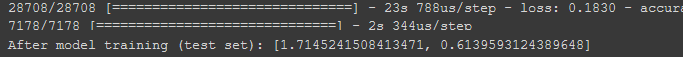
\includegraphics[scale=0.9]{images/modelTwo/evalutaionTwo.png}
Test/Validation Set result is much batter then in prevoius model.\\
\\
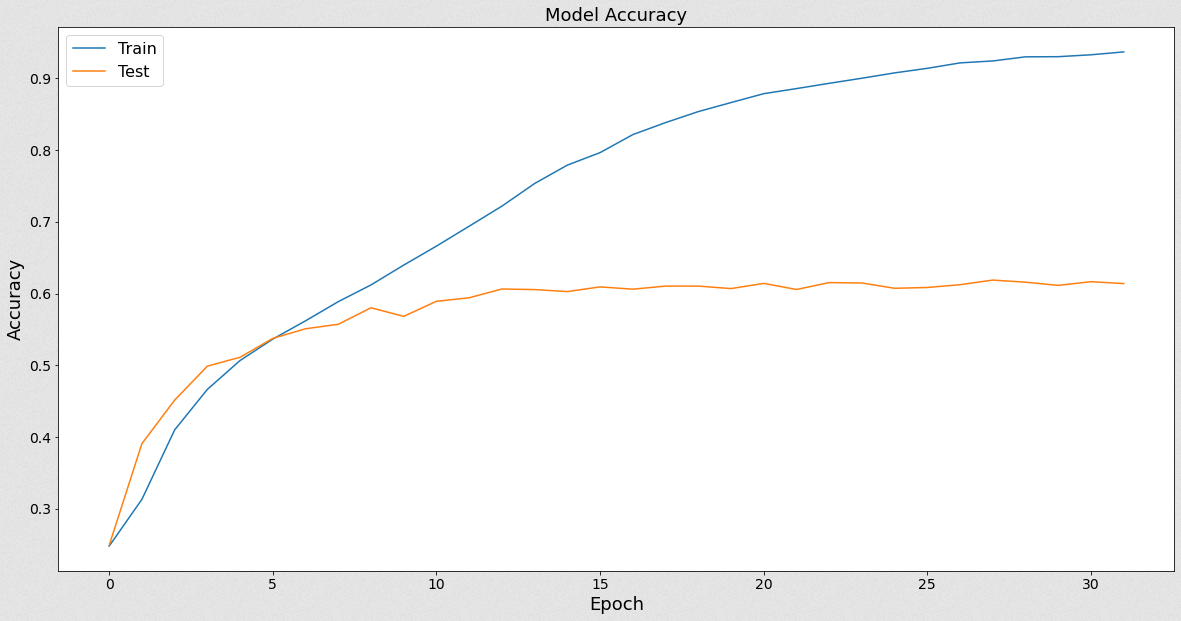
\includegraphics[scale=0.5]{images/modelTwo/accTwo.png}
Accuracy rises as expected.\\
\newpage
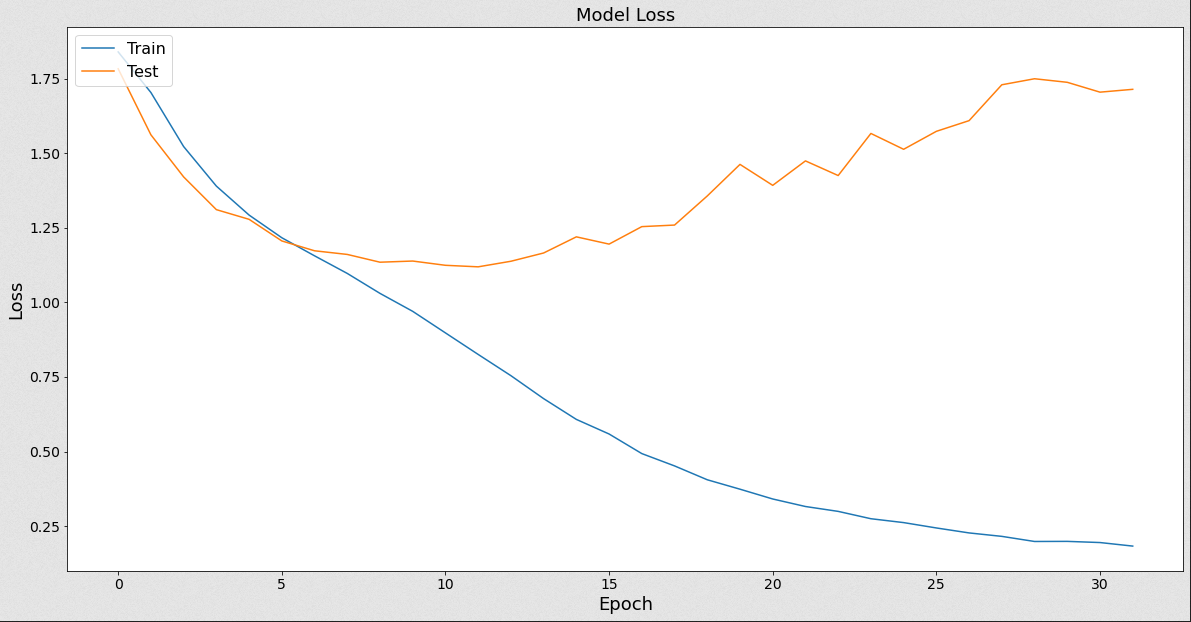
\includegraphics[scale=0.5]{images/modelTwo/lossTwo.png}
Model is over-fitting again but much less.\\
\\
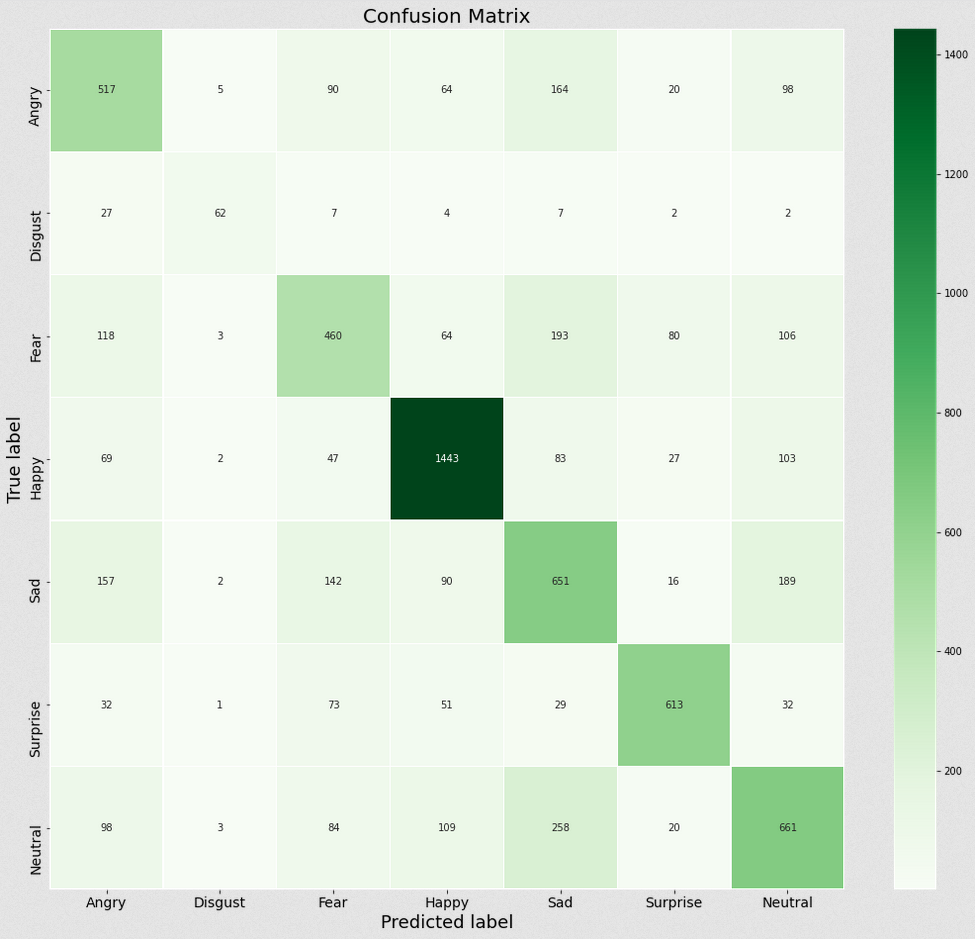
\includegraphics[scale=0.60]{images/modelTwo/matrixTwo.png}
Confusion matrix shows mistakes that model made.\\
\\
Here are some examples:
\begin{itemize}
    \item Correctly predicted images\\
            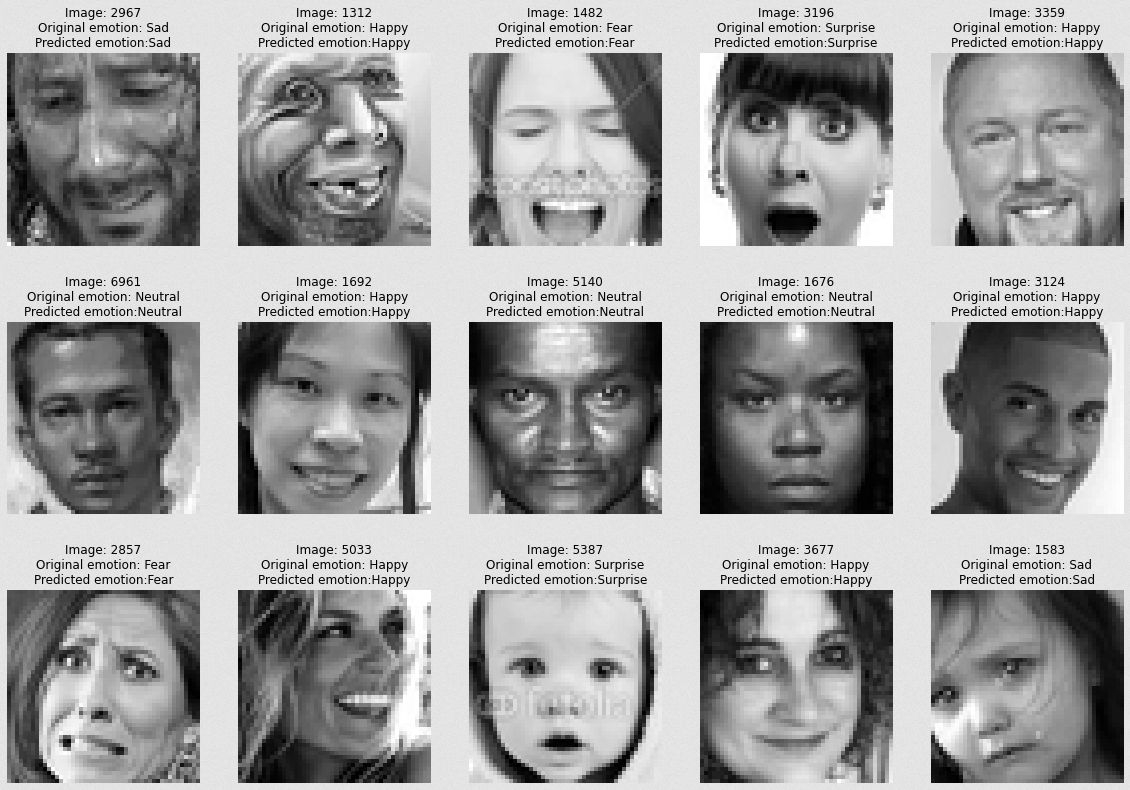
\includegraphics[scale=0.50]{images/modelTwo/trueTwo.png}
    \item Wronly predicted images\\
            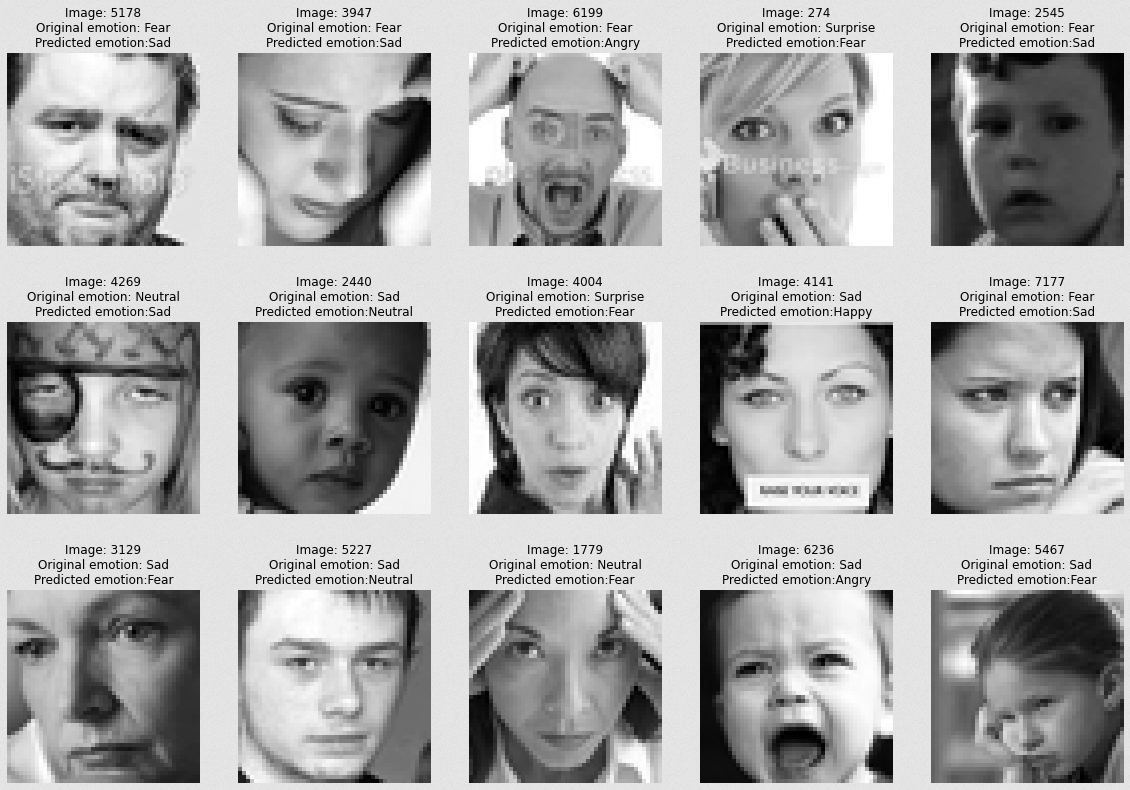
\includegraphics[scale=0.50]{images/modelTwo/falseTwo.png}
\end{itemize}
